\subsection{Effect of the CFO-caused ISI on the BER}
The degradation of BER due only to the ISI introduced by the CFO is shown in figure~\ref{fig:cfoisiber}.
\begin{figure}[htbp]
\centering
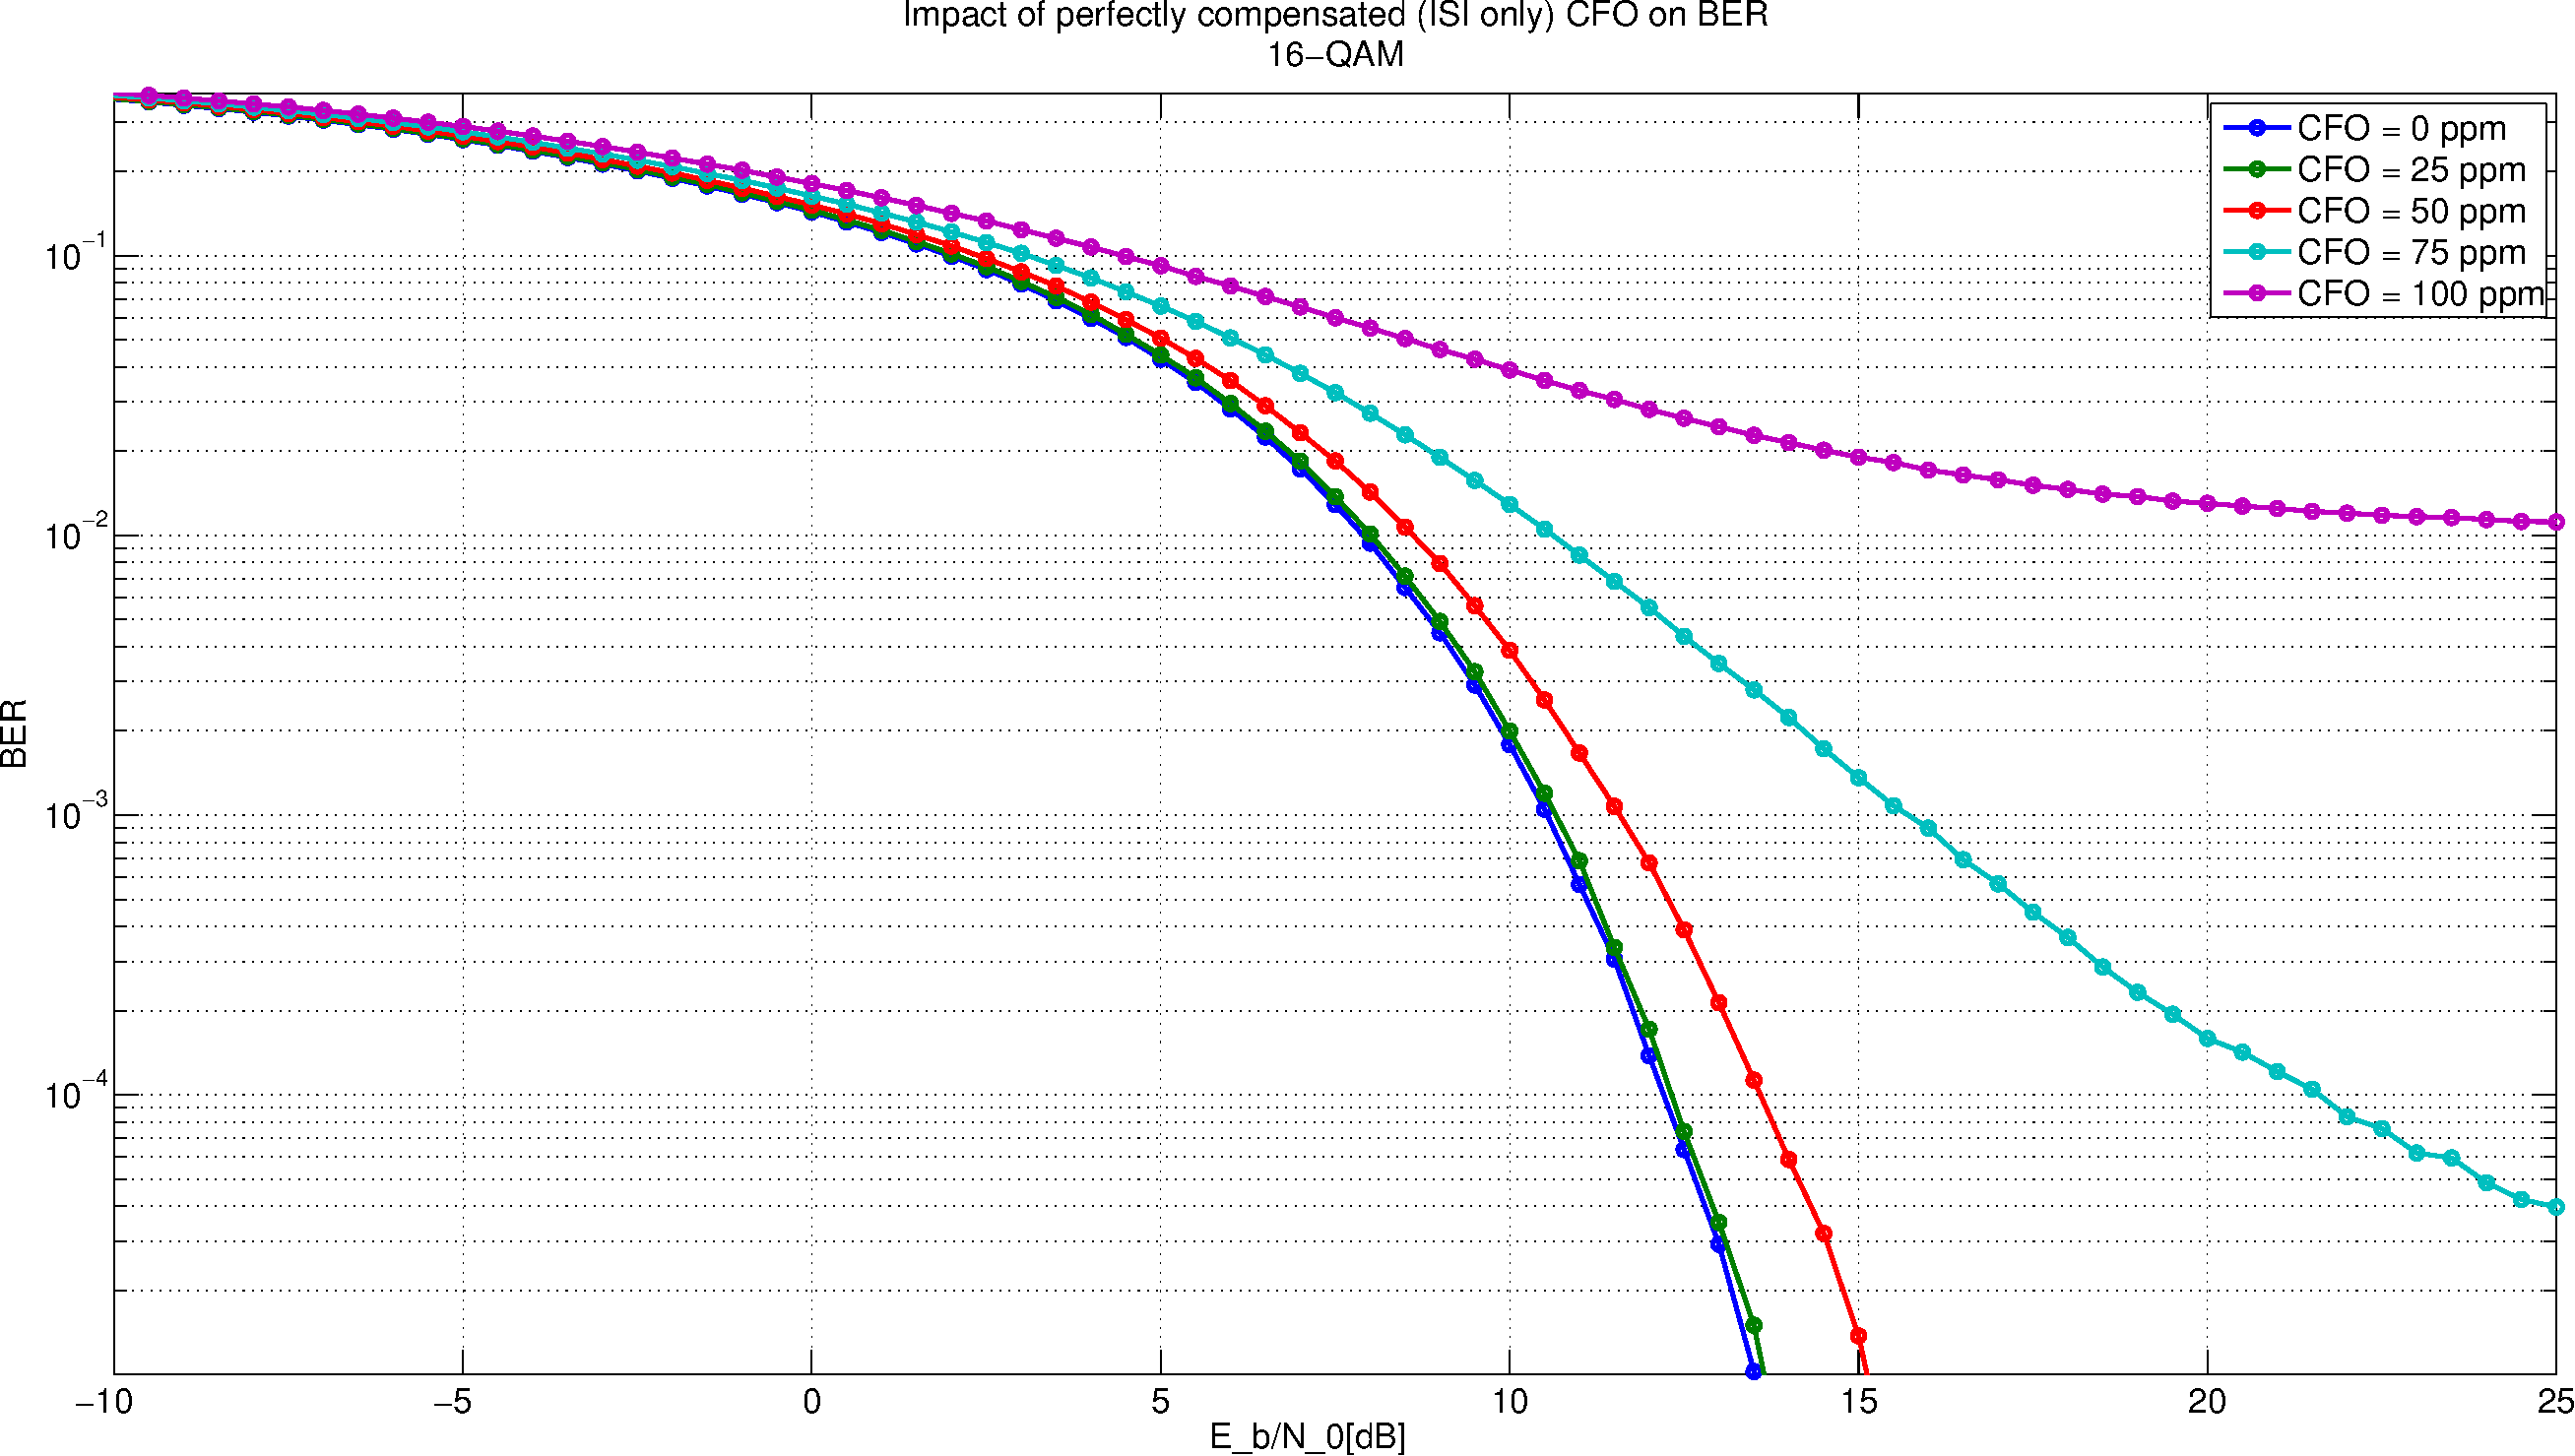
\includegraphics[width=\textwidth]{cfoisiber.pdf}
\caption{Impact of the ISI introduced by the CFO on the BER.\label{fig:cfoisiber}}
\end{figure}
Figure~\ref{fig:cfoisiber} shows that for a given value of $\Delta\omega$ and at higher noise levels, the BER curve is worsened but shows similar behaviour as the original curve with no CFO.
However, past a certain value of $\frac{E_b}{N_0}$, the BER stops decreasing and only the errors introduced by the ISI subsist.
Those plateaus in the curves correspond to what we observed when we were testing the simulation with no CFO but with a misdefined filter which did not cancel the ISI.
To conclude, figure~\ref{fig:cfoisi} shows the ISI of two halfroot nyquist filters separated by CFO.
\begin{figure}[htbp]
    \centering
    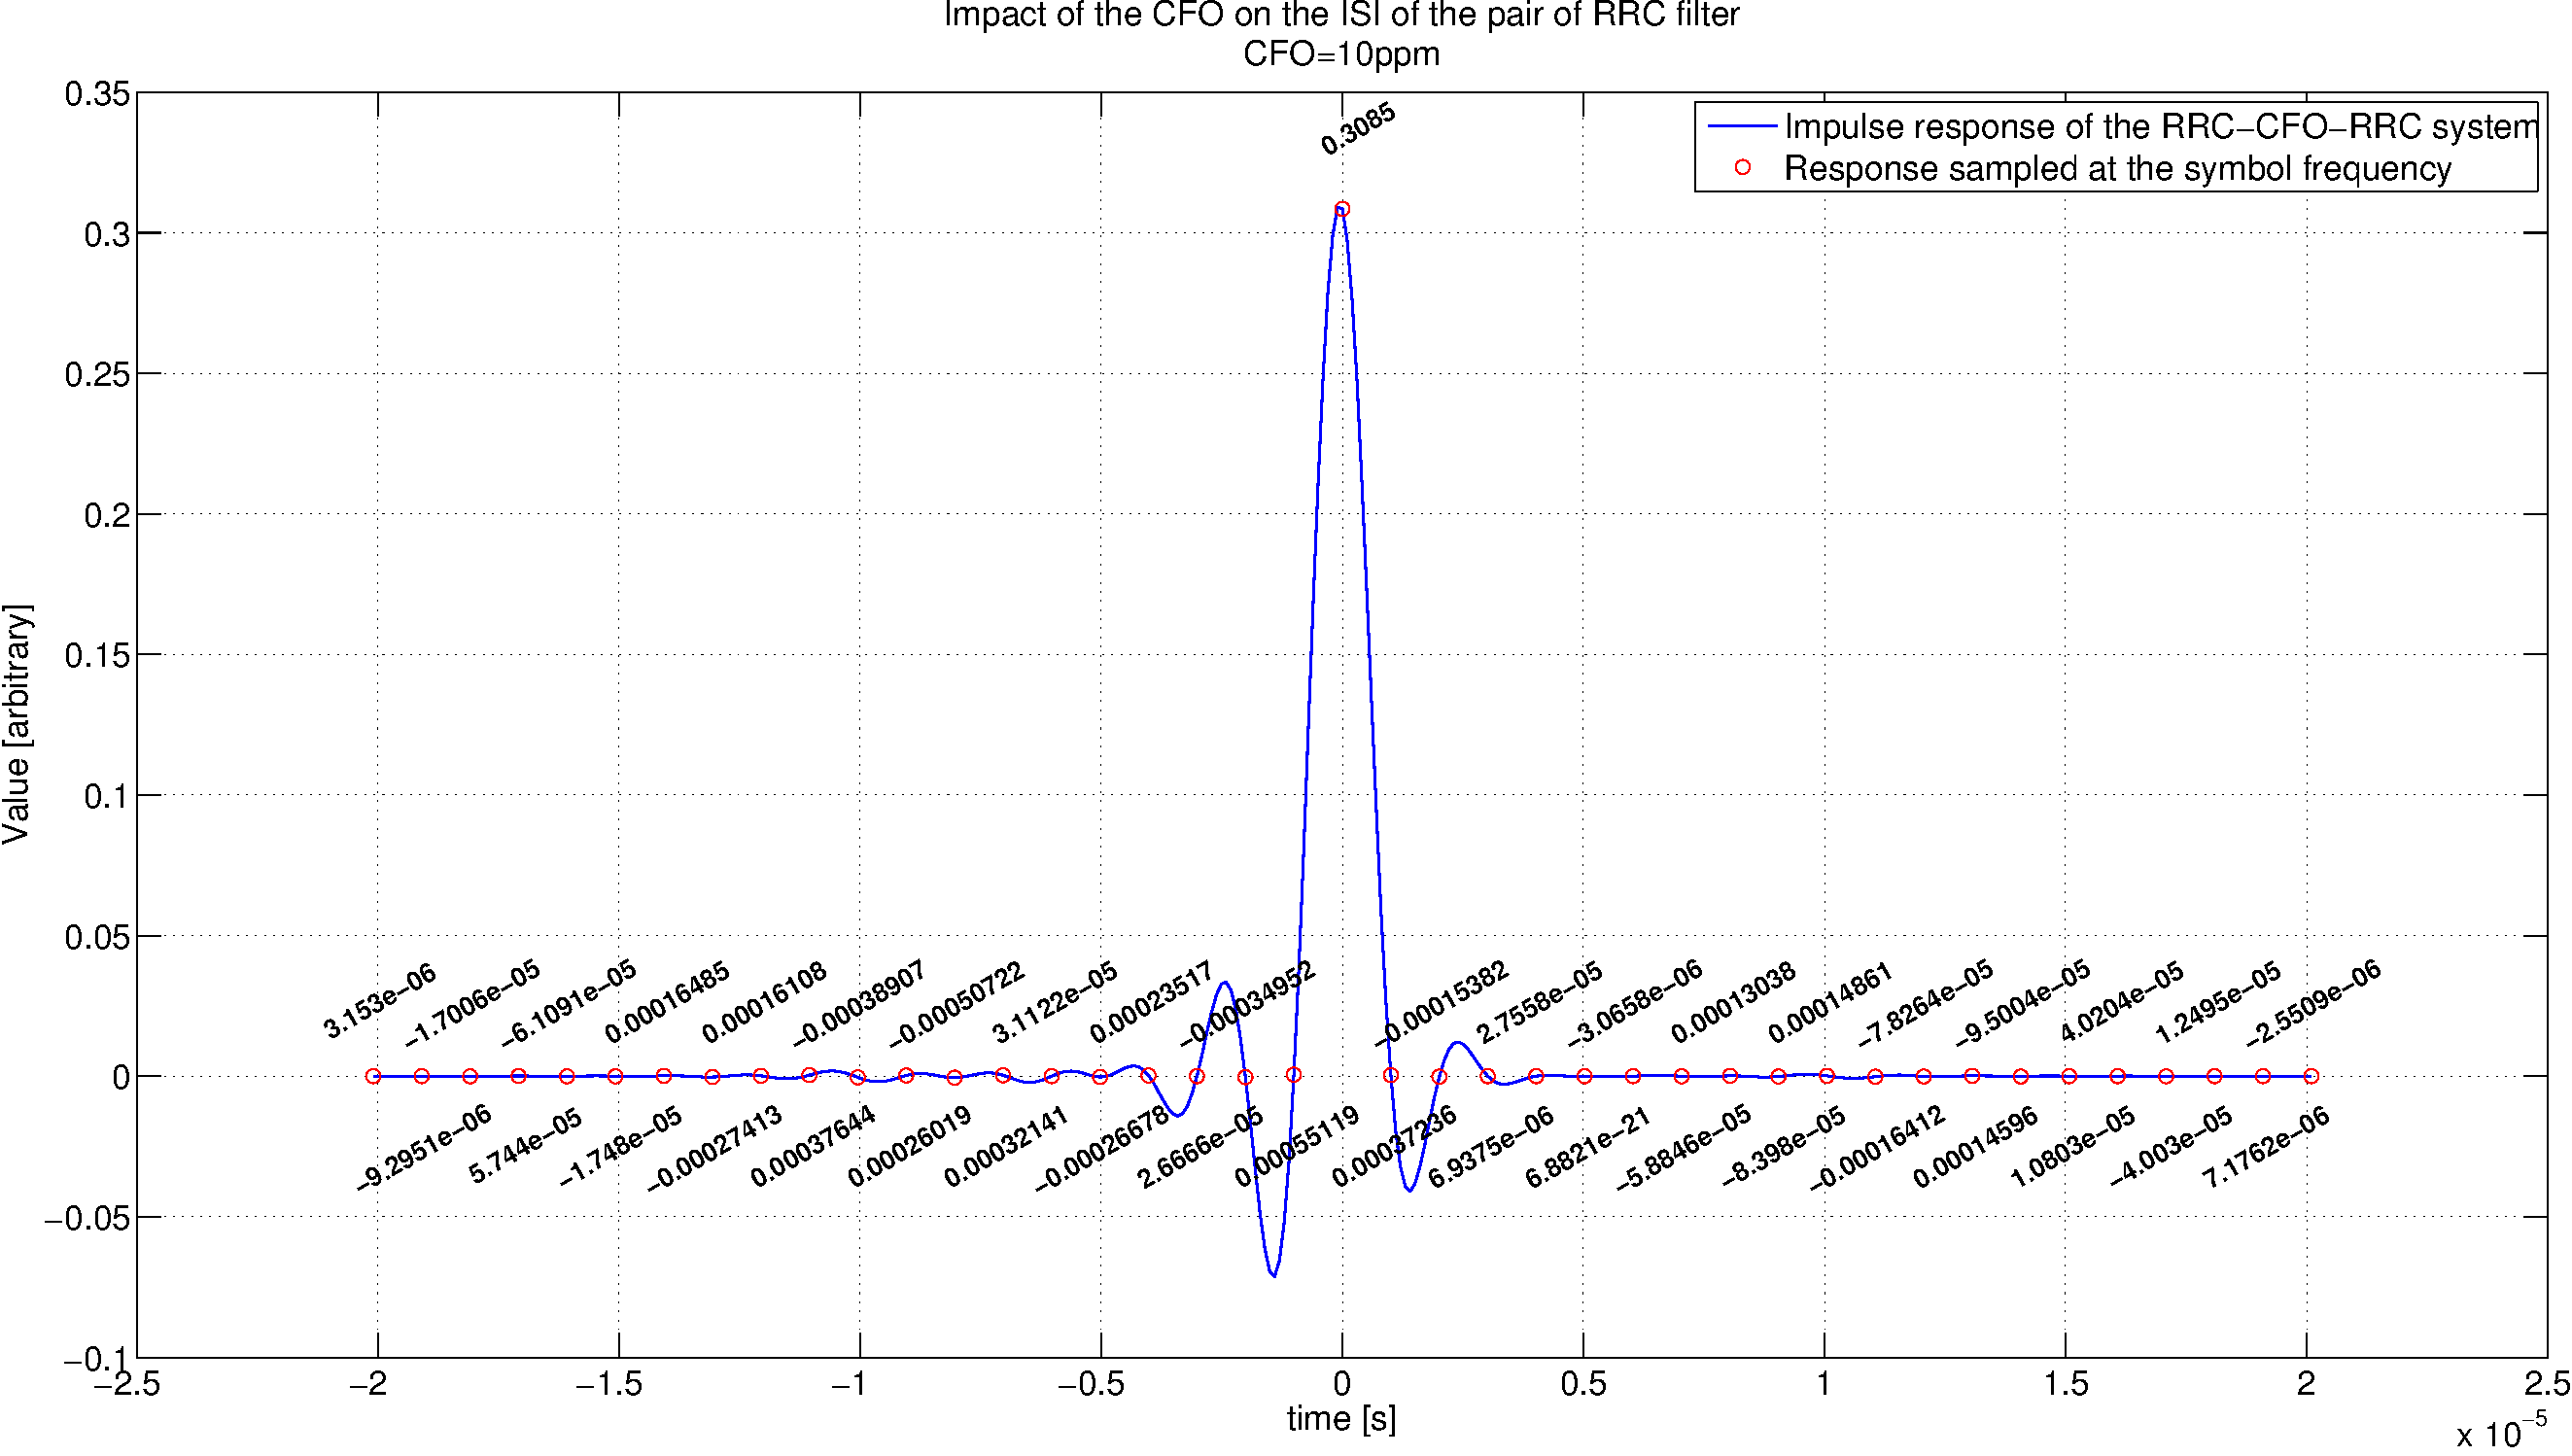
\includegraphics[width=\textwidth]{cfoisi.pdf}
    \caption{Effect of \SI{10}{ppm} of CFO on the ISI of the pair of filters. $\beta = 0.3$, $n_{taps} = 20$, $f_m = \SI{1}{\mega\hertz}$, $f_c = \SI{2}{\giga\hertz}$, $\Rightarrow \Delta\omega = \SI{20}{\kilo\hertz}$.\label{fig:cfoisi}}
\end{figure}

If the cfo is not compensated, the slow phase drift over time renders the channel unusable and BER is 0.5 for any noise levels.

\subsection{Sample time shift error}
Figure~\ref{fig:smpEpsBER} shows the impact of the sample time shift on the error rate.
\begin{figure}[htbp]
\centering
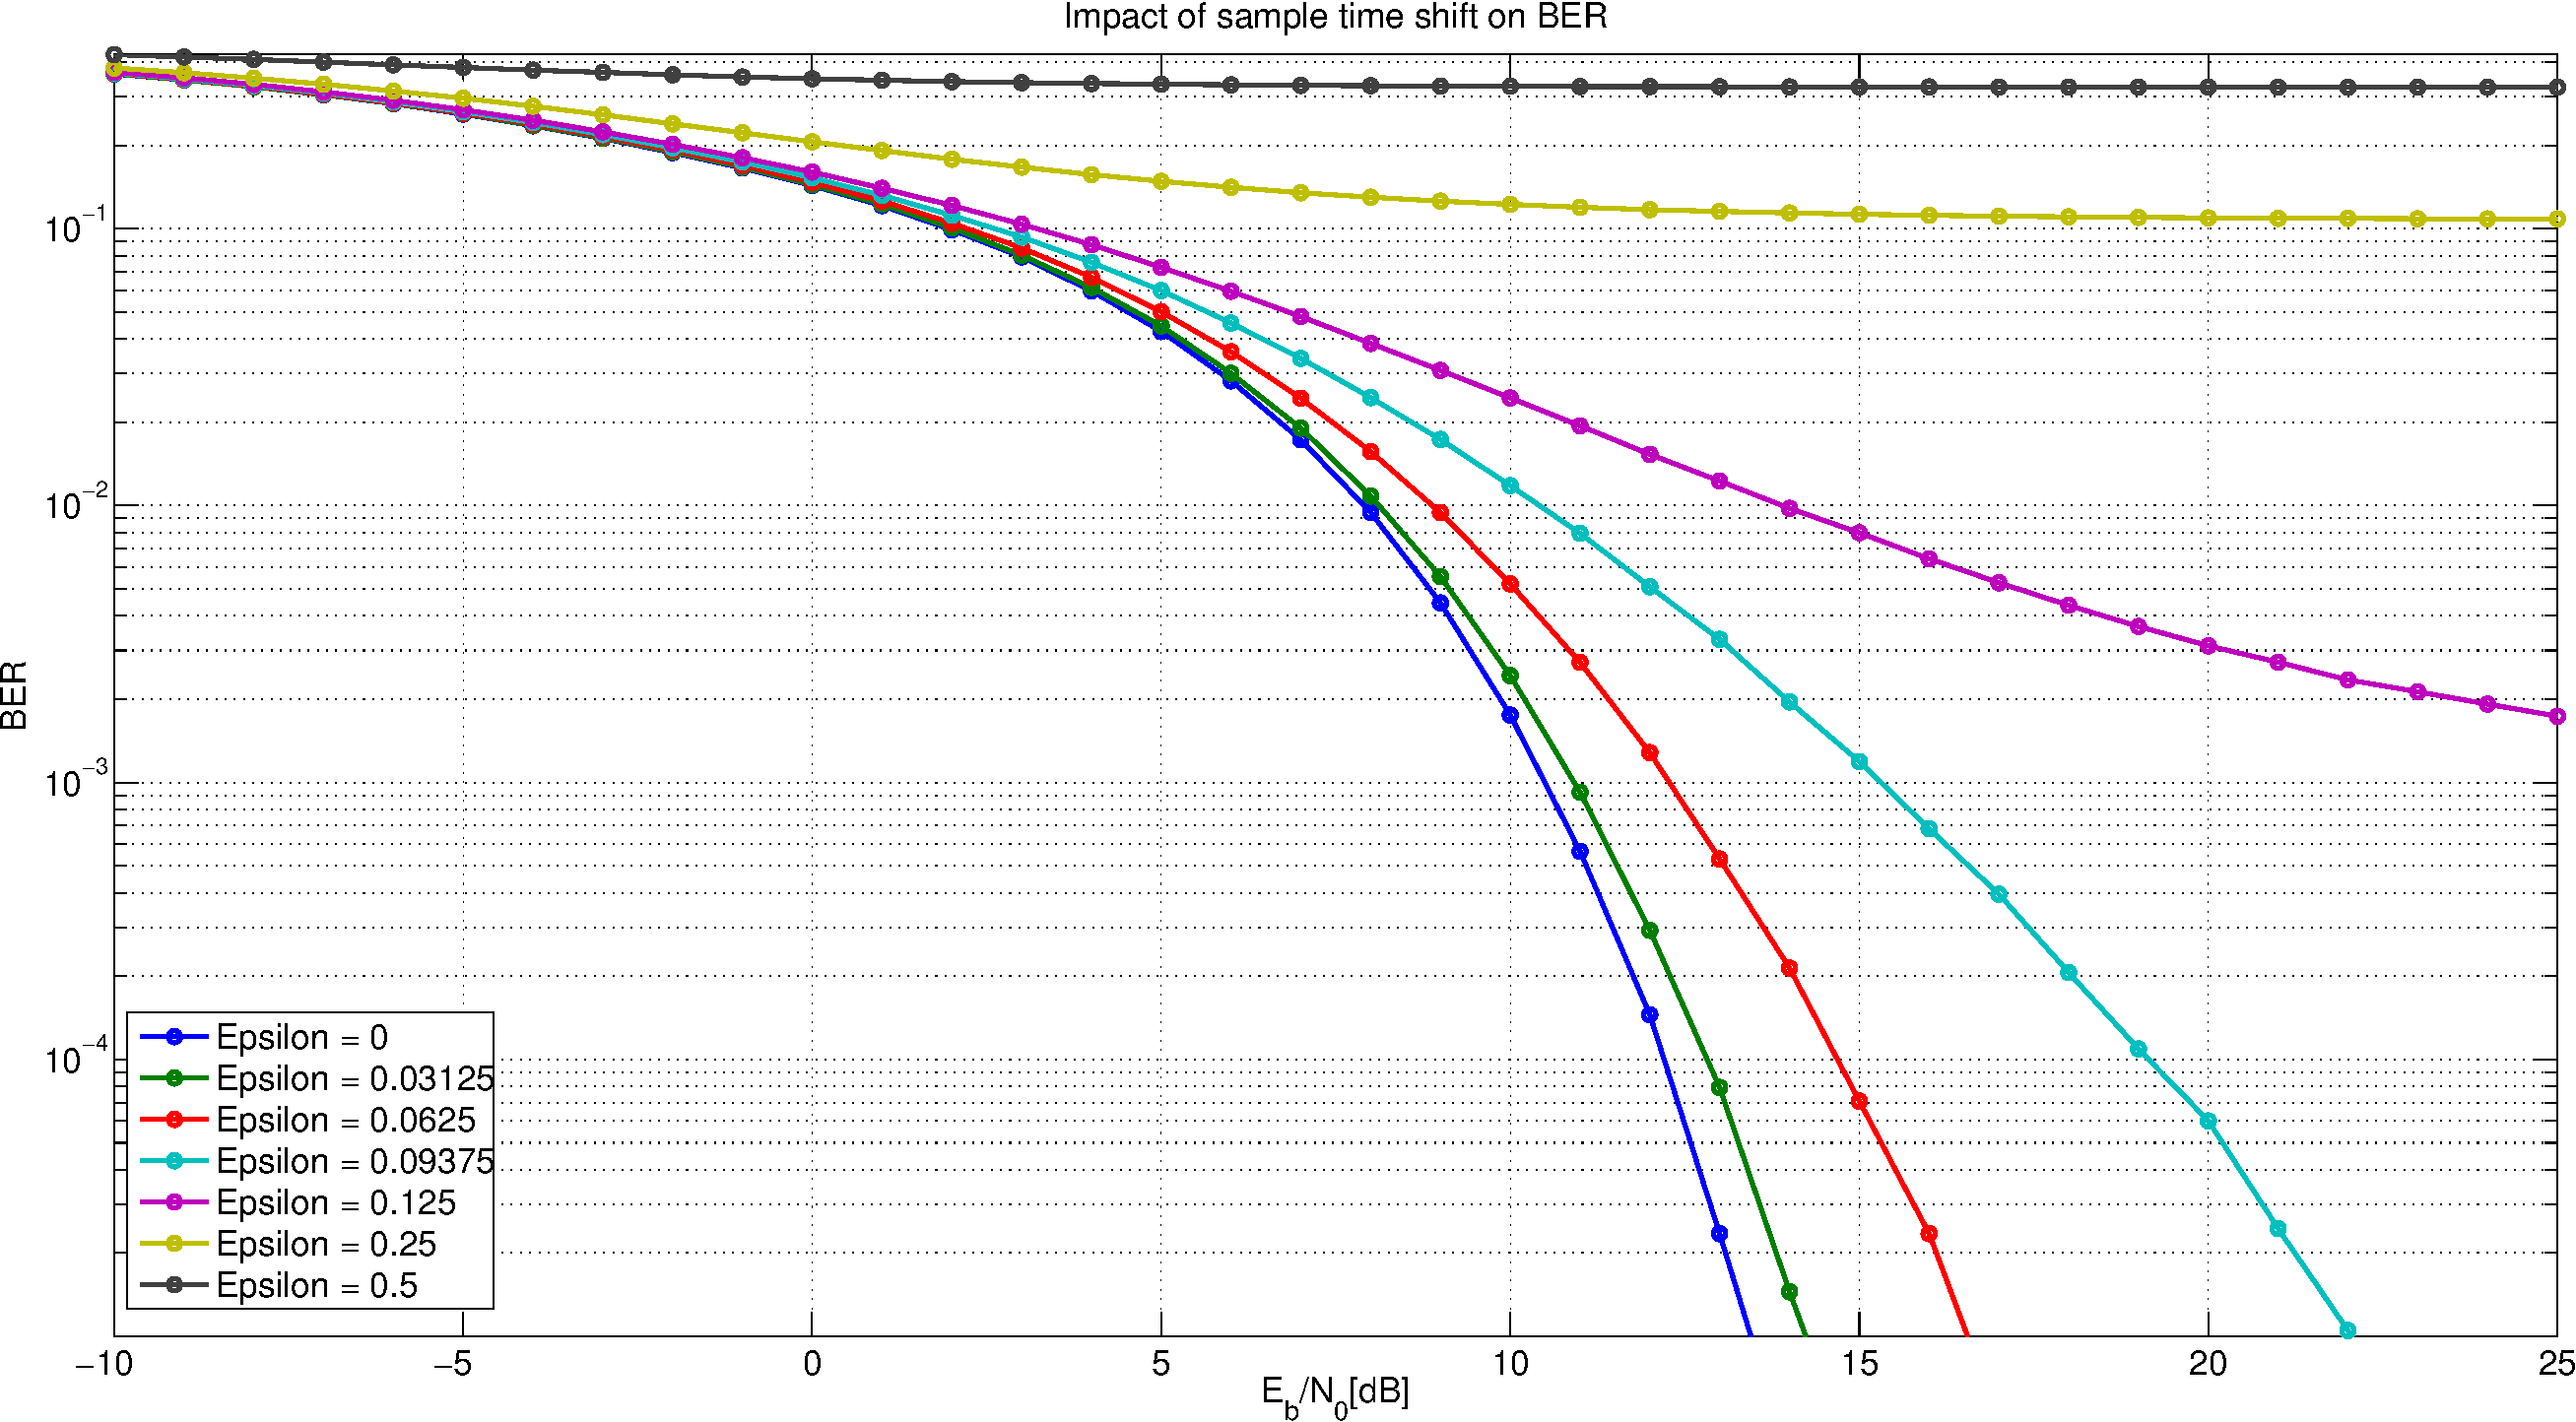
\includegraphics[width=\textwidth]{smpEpsBER.pdf}
\caption{Impact of the sample time shift on the error rate. $f_m = \SI{1}{\mega\hertz}$, $f_s = \SI{32}{\mega\hertz}$ $\Rightarrow \Delta k = 0, 1, 2, 3, 4, 8, 16$ samples\label{fig:smpEpsBER}}
\end{figure}

\subsection{Sample time shift error correction using the Gardner Algorithm}
Figure~\ref{fig:gConvK} shows the convergence of the Gardner algorithm for different error weights.
\begin{figure}[htbp]
    \centering
    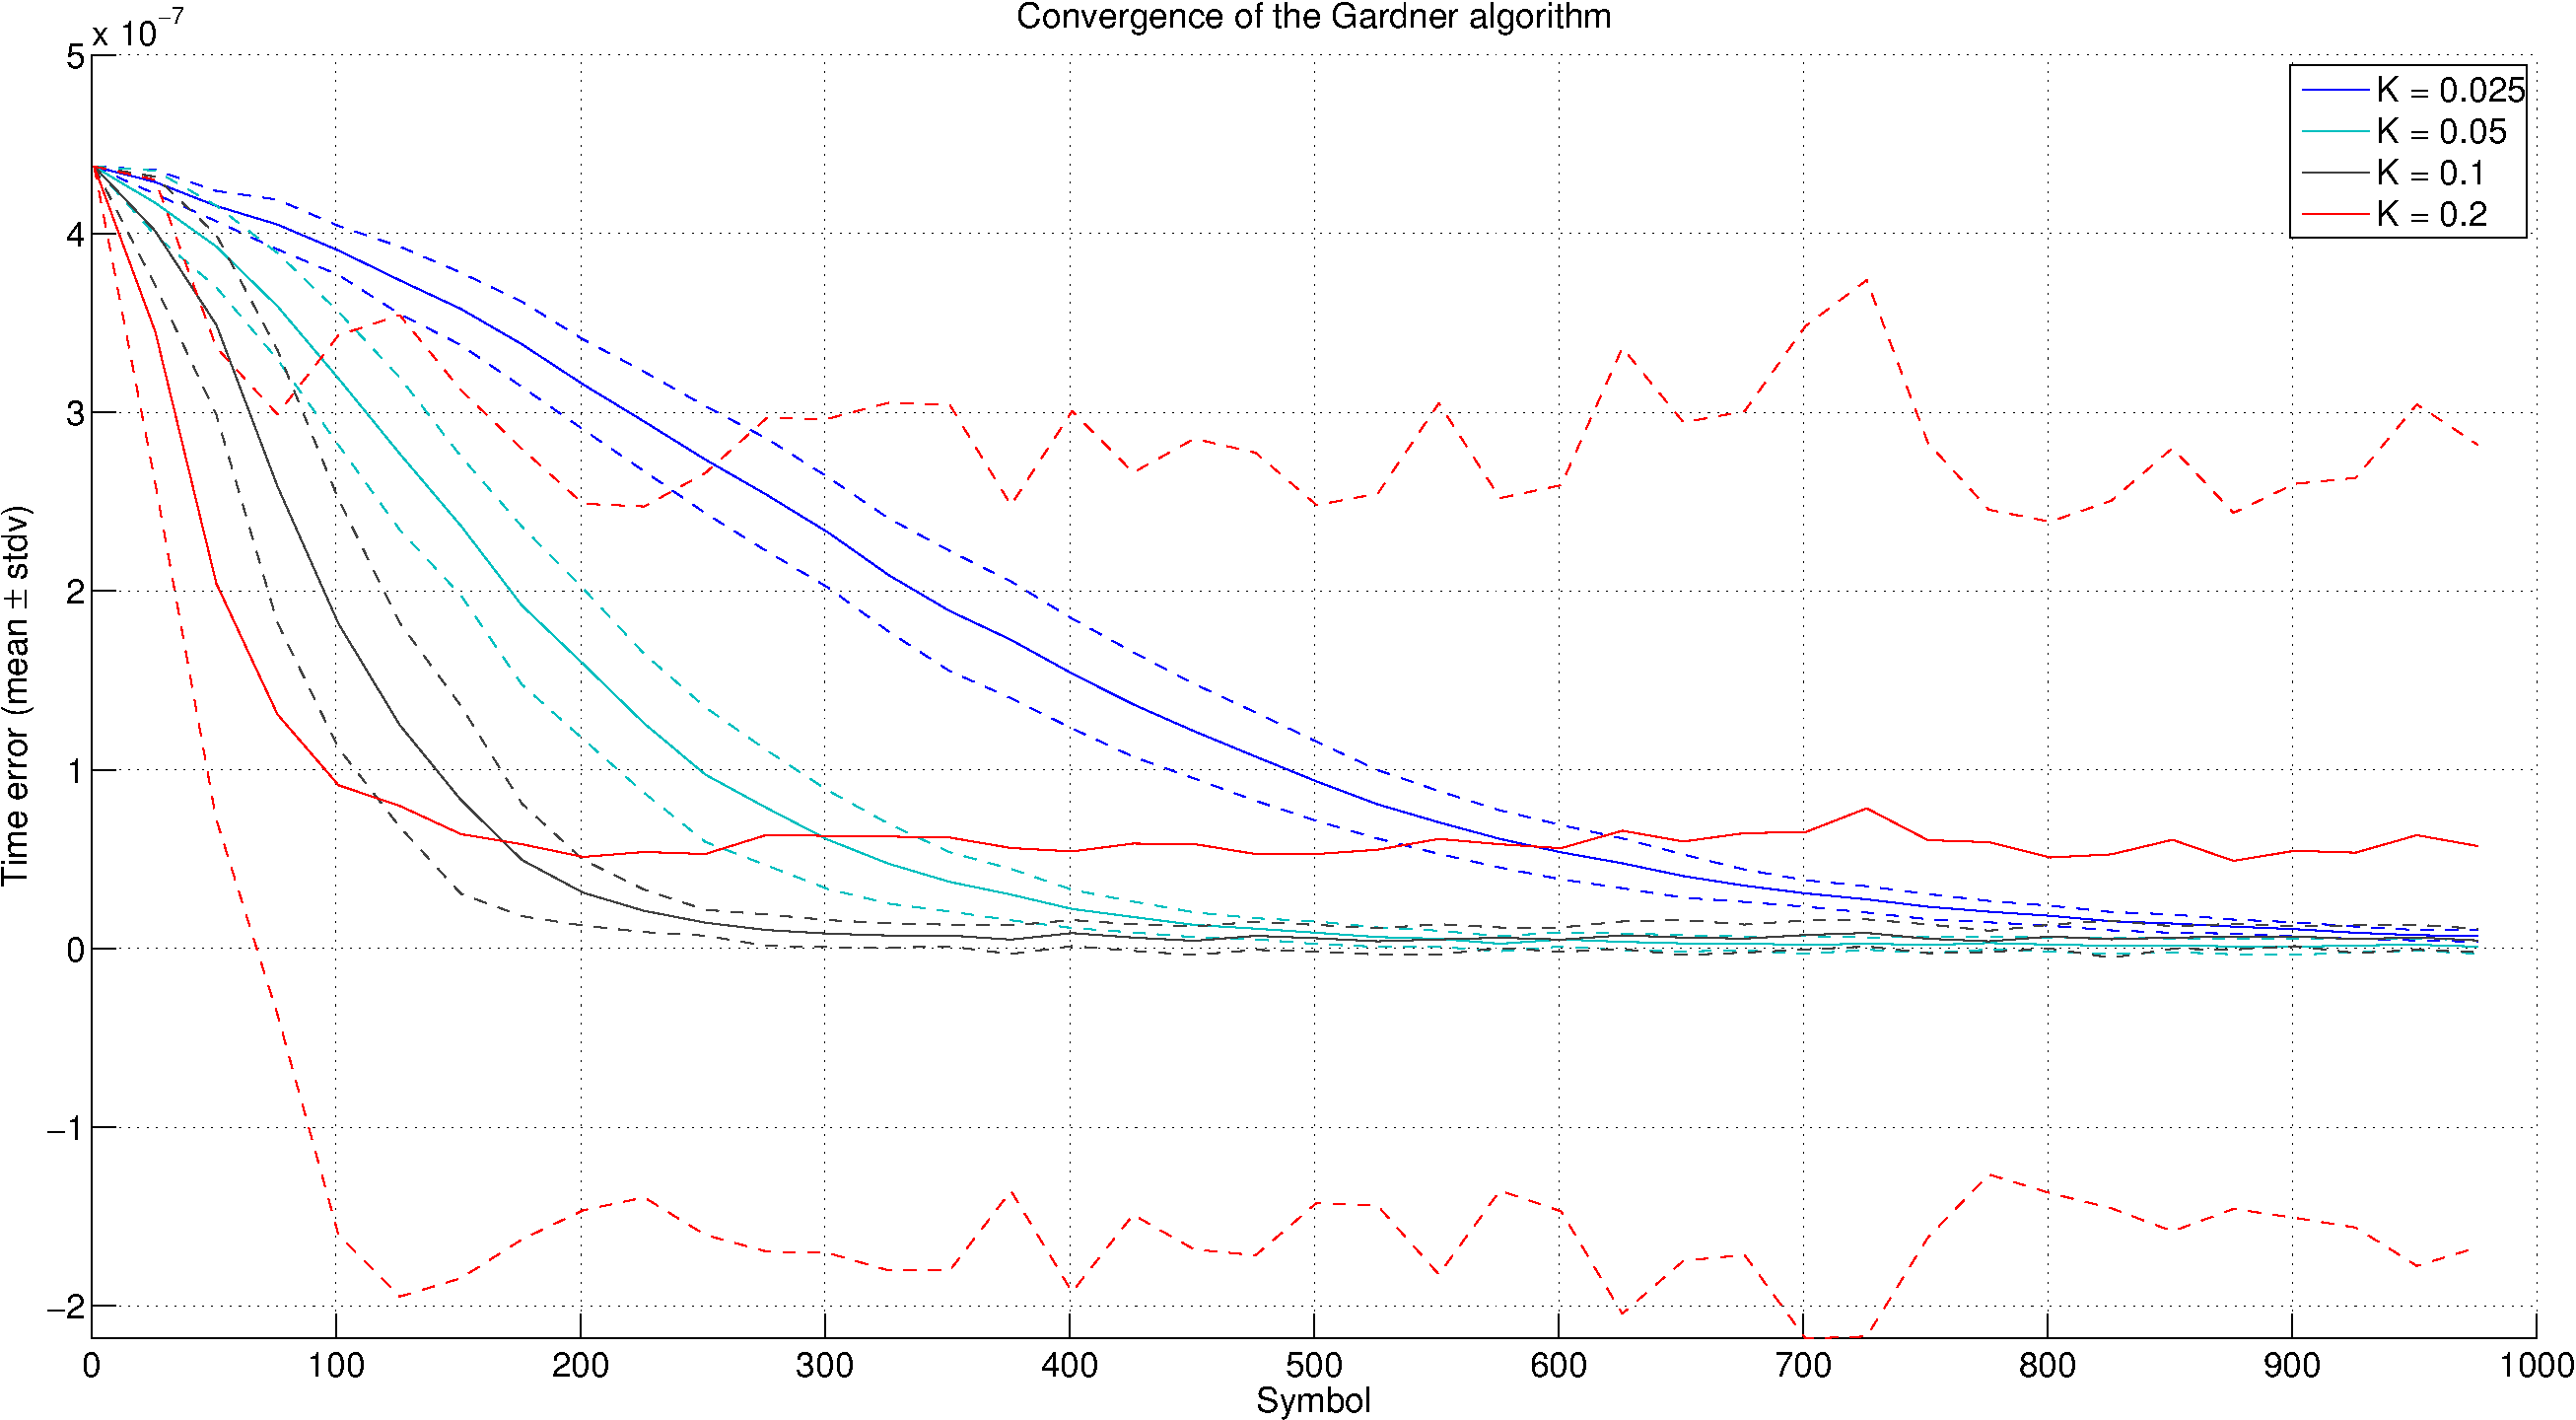
\includegraphics[width=\textwidth]{gardnerConverge.pdf}
    \caption{Convergence as a function of $\kappa$. 4-QAM, $f_m = \SI{1}{\mega\hertz}$, $\beta = 0.3$, $\frac{E_b}{N_0} = \SI{10}{\decibel}$.\label{fig:gConvK}}
\end{figure}

The resistance of the algorithm to CFO is shown in figure~\ref{fig:gConvCFO}.
\begin{figure}[htbp]
    \centering
    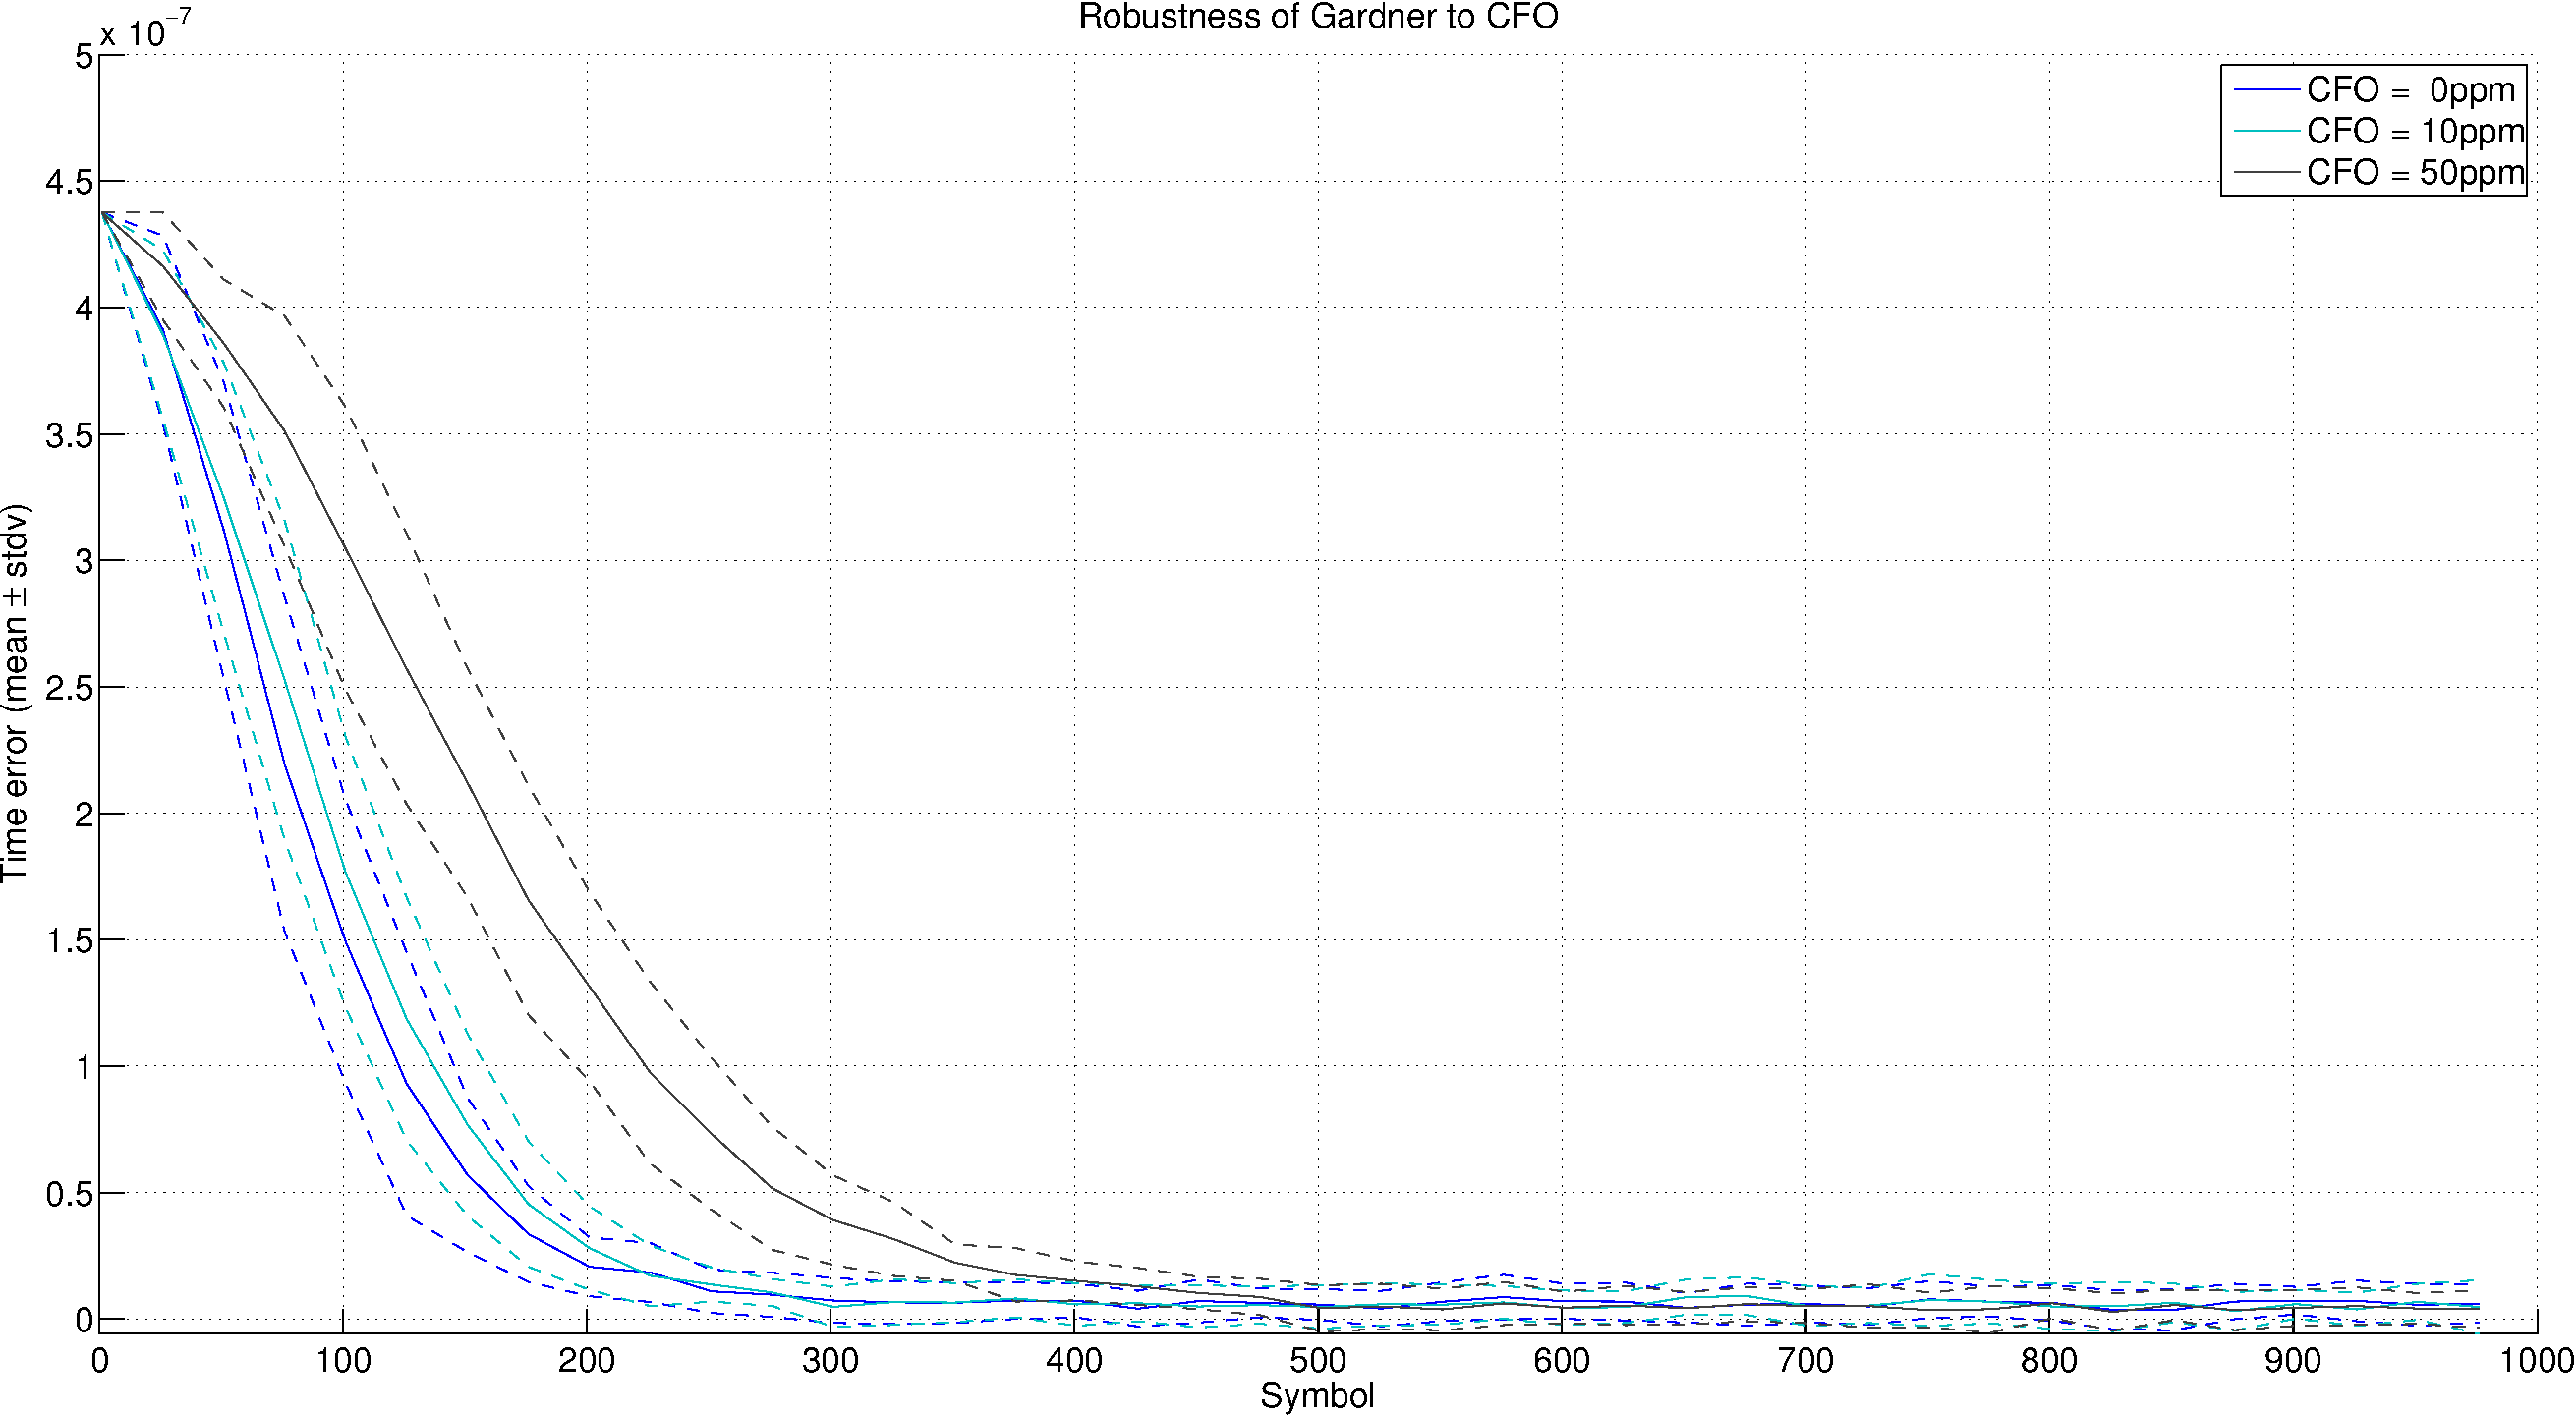
\includegraphics[width = \textwidth]{gardnerCFO.pdf}
    \caption{Convergence of the algorithm as a function of $\Delta\omega$. 4-QAM, $f_m = \SI{1}{\mega\hertz}$, $\beta = 0.3$, $\frac{E_b}{N_0} = \SI{10}{\decibel}$, $\kappa = 0.1$.\label{fig:gConvCFO}}
\end{figure}

\subsection{Questions}
\subsubsection{Simulation}

\paragraph{Derive analytically the baseband model of the channel including the synchronisation errors.}
Derivation: pen and paper.
\begin{figure}[htbp]
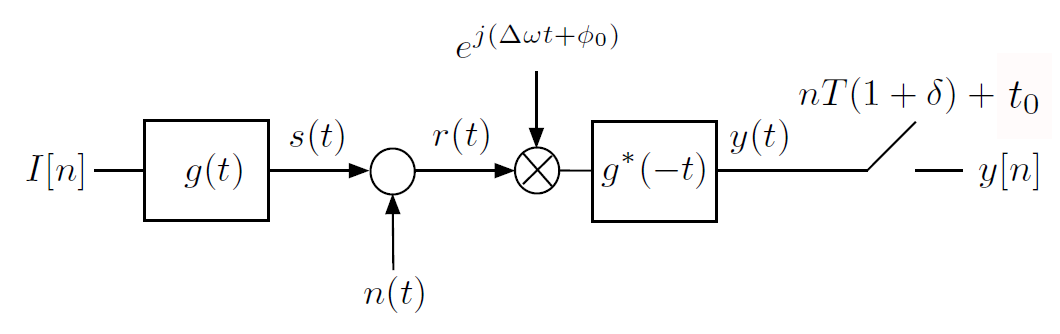
\includegraphics[width=\textwidth]{baseband_sync.png}
\caption{Baseband model with synchronization errors.\label{fig:sync}}
\end{figure}


\paragraph{How do you separate the impact of the carrier phase drift and ISI due to the CFO in your simulation?}
We do this by perfectly cancelling the CFO by hand after the filtering operation at the receiver.

\paragraph{How do you simulate the sampling time shift in practice?}The modulated message at the symbol frequency is first upsampled before all the other operations.
At the receiver, after the filtering operation, is signal is downsampled.
During this downsampling operation, a fixed sampling time shift can be introduced by shifting the indexes.

\paragraph{How do you select the simulated $E_{b}/N_{o}$ ratio?} Typical value is \SI{10}{\deci\bel}. Small enough to get something correct at the end and big enough to get some errors to be able to test our simulated channel with noise.

\paragraph{How do you select the lengths of the pilot and data sequences?} The pilot's length should be long enough to get a good estimation of the phase and the length of the data is selected to ensure a correct phase interpolation between two pilot sequences. Furthermore, the pilot sequence length and repetition should be as small as possible in order to maximize the channel throughput.

\subsubsection{Communication System}


\paragraph{In which order are the synchronisation effects estimated and compensated. Why?} First the sampling time shift is estimated and compensated with Gardner's algorithm, because frame and frequency acquisition can only work on a correctly sampled sequence, while Gardner's algorithm is robust to CFO.


\paragraph{Explain intuitively how the error is computed in the Gardner algorithm. Why is the
Gardner algorithm robust to CFO?} At step n, the time shift error is estimated by looking at the value of the signal between samples n and n-1. If there was a zero crossing, then the middle value should be zero. The estimation of epsilon is then corrected by a term that is proportional to the value of this middle sample.

\paragraph{Explain intuitively why the differential cross-correlator is better suited than the usual cross-correlator? Isn’t it interesting to start the summation at $k = 0$ (no time shift)?}
The differential cross-correlator first estimates the start time, and then the CFO. In doing so, it avoids an exhaustive 2D search which is computationally expensive.

\paragraph{Are the frame and frequency acquisition algorithms optimal? If yes, give the optimisation criterion.}
